\chapter{Umsetzung}
\label{ch:S5_Umsetzung}

\section{Erläuterung des Softwaretechnischen Entwurfs}

Für die Softwaretechnische Umsetzung wurden zunächst die Anforderungen an das Geogameframework in Kapitel \ref{ch4:s:Lösungen} sowie die gewählte Lösung aus Kapitel \ref{ch4:s:choosen_solution} im Detail evaluiert. Für die Umsetzung des Entwurfs wurde zunächst ein Entwurfs des Prozesses identifiziert, welcher die Geodaten aus OSM bis hin zur Darstellung im Beispielspiel darstellt. Eine Visualisierung ist in Abbildung \ref{img:ch5_img01_framework_progress} zu sehen.
\\\\

\begin{figure}[H]
\begin{center}
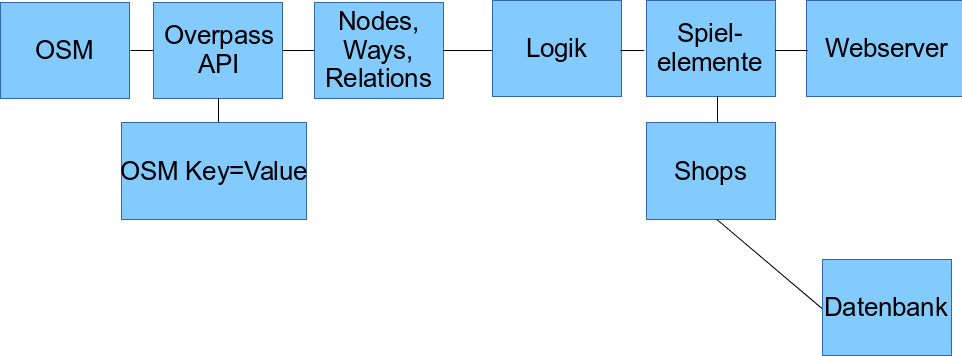
\includegraphics[width=140mm]{images/ch5_img01_framework_progress.png}
\caption{Prozess: Von OSM zum Spielelement}
\label{img:ch5_img01_framework_progress}
\end{center}
\end{figure}

\subsection*{OSM und Overpass API}

Zunächst steht zu Beginn des Prozess als Datengrundlage Openstreetmaps.
Die Daten werden allerdings nicht direkt von OSM über die OSM API abgerufen, sondern über Overpass. Das liegt daran, dass die OSM API selbst nur sehr rudimentäre Abfragen erlaubt.
Stattdessen wird die Overpass API verwendet, da diese geografische Abfragen erlaubt \cite{Meyer.2013}.
Diese Abfragen sind notwendig, um die zuvor deklarierte Anforderung, die Spielelemente basierend auf einem OSM key-value Paars zu bewerkstelligen. Darüber hinaus wird die Transformation der Relations und Ways in Nodes einfacher ermöglicht.
Durch die Verwendung der Overpass QL-Abfrage Sprache (OQL) ist es möglich sich nicht nur die jeweiligen Relations, Ways und Nodes eines tags zu erhalten, sondern auch zusätzlich alle rekursiv enthaltenen Elemente. Dies ermöglicht es den kompletten Datensatz mit einer Abfrage zu erhalten der für die spätere Transformation benötigt wird. Der Vorteil liegt darin, dass nicht mehrere Abfragen gestartet werden müssen und somit die Zeit bis alle Daten zur Verfügung stehen erheblich reduziert wird. Die Overpass API selbst bietet diverse Ausgabe Formate wie XML und JSON \cite{Olbricht.2014}. Für eine konkrete Umsetzung wurde sich bewusst für JSON entschieden, da zum einen die Performance bei der Verabreitung von JSON Dokumenten beachtlich höher ist im Vergleich zu XML Dokumenten \cite{Nurseitov.2009}. Zum anderen soll die Daten später als GeoJSON aufbereitet werden.
Der Aufruf der OverpassAPI erfolgt mittels einfacher REST-Abfrage:
\\\\
\url{http://overpass-api.de/api/interpreter?data=OQL_BEFEHL}
\\\\
Über den Parameter "data" wird der jeweilige OQL Befehl abgesetzt.
Für die Weiterverarbeitung der Daten wird im Anschluss das JSON Ergebnis vom Framework geparst und weiterverarbeitet.

\subsection*{Transformations Logik}

Die Transformation der Relations und Ways wird wie in Kapitel \ref{ch4:s:choosen_solution} umgesetzt. Eine Visualisierung ist in Abbildung \ref{img:ch5_img02_transform} zu sehen.

\begin{figure}[H]
\begin{center}
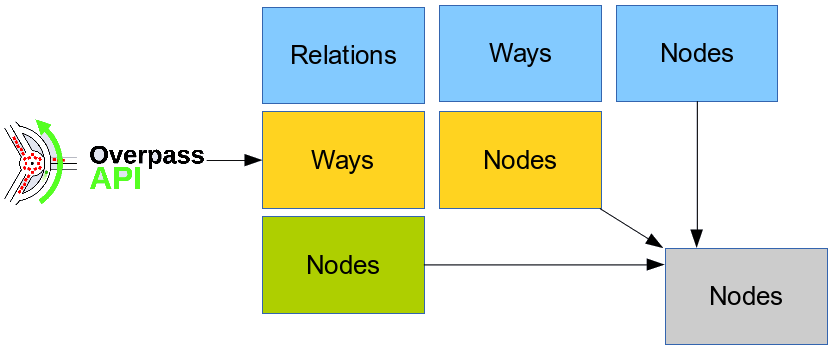
\includegraphics[width=140mm]{images/ch5_img02_transform.png}
\caption{Transformationsprozess: Relations, Ways, Nodes}
\label{img:ch5_img02_transform}
\end{center}
\end{figure}

Auf der linken Seite sind vertikal die Ausgangstypen angeordnet. Hierbei handelt es sich um die bereits angesprochenen Elemente Relations, Ways und Nodes. Im zweiten Schritt, nach dem Aufbereiten der Daten von der Overpass API wird wie folgt vorgegangen. Zunächst werden alle Relations behandelt, im Anschluss darauf die Ways und zum Schluss die Nodes. Die Idee dahinter ist es zunächst alle Ways und Nodes zu identifizieren welche direkt einer Relation angehören und keine separaten Spielelemente darstellen. Die Vorgehensweise ist damit begründet, dass durch die Reduzierung der Anfrage auf ein einzelnen Request die Rückgabe alle Nodes enthält. Sowohl die Nodes einer Relation, als auch die eines Ways, welche selbst nicht eigenständig sind. Daher müssen die Elemente Ebene für Ebene wie in der Abbildung zu sehen, abgearbeitet werden.
\\\\
Zunächst werden alle Relationen identifiziert. Für jede Relation werden nun die beinhalteten Ways und Nodes identifiziert. Diese wiederum werden dann als "gecalaimed" markiert. Relations selbst werden nicht rekursiv aufgelöst, da das Ziel nicht ist möglichst wenige Spielelemente zu haben, sondern Relationen zu transformieren. Sollten Relations mehreren Unterrelations haben so sollen diese als Eigenständige Elemente betrachtet werden. Sofern dieser Ansatz sich als Nachteilig in der Evaluation herausstellt muss er entsprechend modifiziert werden.
Für die jeweilige Iteration eines Relation Elements werden nun alle beteiligten Ways und Nodes zu einer Liste von Nodes zusammengefasst, Diese Liste wird wiederum durch das in Kapitel \ref{ch4:s:choosen_solution} beschriebene Verfahren einer Bounding Box dessen Mittelpunkt berechnet wird reduziert auf ein virtuelles Node, welches die Relation repräsentiert. Dieses virtuelle Node hat eine Koordinate, sowie eine ID welche eindeutig identifizierbar ist. Hierzu wird die Relations ID von OSM verwendet.

Im nächsten Schritt werden die Ways abgearbeitet. Bereits als "geclaimed" markierte Ways, die somit bereits in einer Relation enthalten sind, werden ignoriert. Alle anderen Ways werden entsprechend jeweils wiederum zu einer Liste von Nodes und anschließend zu einem virtuellen Node transformiert. Hierbei entsteht wieder eine Koordinate und als ID wird die OSM Way ID verwendet.

Die Elemente, welche direkt als Node zurückgegeben werden analog übernommen. Sie werden in Spielelemente, hier durch das graue Nodes Element symbolisiert, transferiert. Hierzu wird die Koordinate, sowie die OSM ID der Nodes übernommen.

Eine Problematiks tellt sich allerdings noch in der eindeutigen Identifizierung der virtuellen Nodes. Da diese von unterschiedlichen Elementen (Relatons, Ways, Nodes) abgeleitet wurden muss sichergesteltl werden, dass anhand der ID eine eindeutige OSM Zuordnung möglich ist.
Entweder es wird zusätzlich der abgeleitete typ des Spielelements explizit gespeichert oder aber, man transcodiert die Information mit in die ID.
Wenn man sich zunächst die OSM IDs für Nodes anschaut, stellt man fest, dass diese die 32bit signed Integer Grenze überschritten haben (Februar 2013). Im OSM Wiki wird daher empfohlen den Datentyp long zu verwenden, welcher in den Standard-Implementierungen ein 64bit Wert ist \cite{OSM.2013b}.
Eine Methode um den Typ des Spielelements zu übertragen könnte mit einer Bitmaske der ID funktionieren. Hierzu könnte man die den 2. und 3. Bit Bits des 64bit Wertes verwenden. Der 1. it wird nicht verwendet um negative Zahlen weiterhin zu erlauben. Der 2. Bit würde als Identifikator für Relations dienen und der 3. für Ways als Ursprungselement. Ein Beispiel für den transformierten Way mit der OSM ID 1 ist in Abbildung \ref{img:ch5_img03_bitmask} zu sehen.

\begin{figure}[H]
\begin{center}
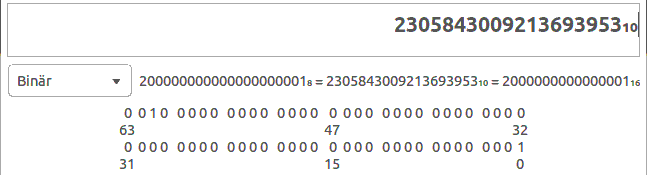
\includegraphics[width=120mm]{images/ch5_img03_bitmask.png}
\caption{OSM ID: Bitmaskenkodierung im 64bit long Wert}
\label{img:ch5_img03_bitmask}
\end{center}
\end{figure}


Wenn man die Reduzierung von 63bit (signed) auf 61bit(signed) mit der aktuellen Mapping Geschwindigkeit bei OSM vergleicht, so lässt sich feststellen, dass die Reduzierung um 2 bit aus Paradigmensicht zwar unsauber erscheint, aber eine Überschreitung der ID \begin{math}2^{61}\end{math} in ferner Zukunft liegt. Zudem könnte im Bedarfsfall wenn OSM auf 128bit IDs umsteigt die Bitmaske entsprechend angepasst werden.

\subsection*{Händler Integration}

Nachdem die virtuellen Nodes für die Spielelemente alle erstellt wurden, müssen die Elemente um die Händlern ergänzt werden. In Kapitel \ref{ch4:s:choosen_solution} wurde erläutert, dass die Händler nicht als aktives Spielzielelement verwendet werden sollen, sondern eine Integration der Händler und Dienstleister im Spiel als Repräsentation ihrer Selbst. Die Händler fungieren in diesem Zusammenhang als Anbieter für Items und andere Gegenstände. Für die spätere Darstellung auf der Karte müssen diese ebenfalls mit einer Koordinate versehen werden und separat behandelt werden. D.h. die Spielpunkte der Händler kommen stattdessen aus einer lokalen Datenbank. Dabei wird bewusst auf die Verwendung von OSM Als Basis verzichet. Zwar könnte man in einer erweiterten Version des Frameworks dem Nutzer unterstützen mit automatischen Vorschlägen basierend auf OSM, jedoch ist dies in der Grundfunktion nicht notwendig. Hier soll der Händler sich beliebig frei auf der Karte Positionieren können und entsprechende Parameter seines virtuellen Geschäfts festlegen. Im Anschluss soll er entsprechende Items in seinem virtuellen Shop hinterlegen können. Da die Items eventuell vom Händler gegen einen Betrag vom Spielleiter erkauft werden, hat der Spielleiter ein gewisses Interesse, dass er zum einen die Items im Spiel möglichst an die Spieler bringt, während er auf der anderen Seite das Spiel nicht in einen nicht balancierten Zustand bringt. D.h. dass eventuell zu viele Spieler durch die Nähe eines Händlers mit einem sehr nützlichen Item bevorzugt werden. Daher sollte es im Ermessen des Spielleiters liegen, dass dieser die Art und Verwendung der Items selbst definiert und entsprechende Vorschläge für die Händler parat hat. Dass der Händler selbst sich mit Spielmechaniken und Balancing auseinander setzt ist höchst unwahrscheinlich und würde auch nur zu extra Koordinationsaufwand führen. Daher ist es am sinnvollsten dem Händler gewisse Items mit standard Eigenschaften anzubieten, von denen er einen Typ selbst auswählt und eine entsprechende Menge seinem virtuellen Shop zuordnet.
Für die Itemtypen kann der Spielleiter aller Voraussicht nach auf gewisse Grunderfahrungen zurückgreifen. Darüber hinaus sollte das Framework ihm zu einem späteren Zeitpunkt in einer erweiterten Ausbauphase auch entsprechendes Feedback über die Verwendung und Nutzung der Items aufzeigen und der Spielleiter somit aufgrund dieser Information Rückschlüsse auf das Balancing machen kann.

\subsection*{Persistenz}

Ein wichtiger Aspekt des Frameworks stellt die Persistenz dar. Es müssen die Spielelemente, sowie der Spielzustand selbst gespeichert werden. Die Daten für die Spielelemente stammen aus OSM und von der lokalen Datenbank. Da die OSM Daten entsprechend transformiert werden stellt sich die Frage ob dieser Prozess beschleunigt werden kann, wenn die Daten entsprechend in der Datenbank lokal zwischengespeichert werden.
In Kapitel \ref{ch4:s:choosen_solution} ist bereits auf diesen Aspekt eingegangen worden. Die Problematik die sich durch eine Zwischenspeicherung stellt ist zum einen die Aktualisierung der Daten. Die lokalen Daten müssten mit einem Zeitstempel versehen werden und gehalten werden, bis diese "verfallen". Darüber hinaus müssten diese nach dem Verfallszeitpunkt entsprechend gelöscht oder aktualisiert werden oder belassen werden. Ein Caching kann hier Sinn sofern das Framework für ein Spiel mit einer kritischen Masse an Spielern verwendet wird. Allerdings ist eine Evalutation und Untersuchung des Frameworks auf Hochskalierbarkeit nicht Bestandteil der ersten Ausbaustufe. Ein weiterer Aspekt stellt die Datenmenge dar. Sofern im Framework alle jemals abgefragten OSM Daten in virtuellen Nodes/Spielelementen in der Datenbank hinterlegt werden ohne dass diese eine Zustandsveränderung erfahren haben ist dies zwar Modelltechnisch korrekt, allerdings aus Performance und Platzgründen nicht zu empfehlen. Speziell in der Hinsicht, dass das Framework dem Spielleiter so wenig Aufwand wie möglich machen soll, sollte verhindert werden, dass der Spielleiter sich um Datenbank und Speicherplatz Probleme kümmern muss. Ein gutes Beispiel hierfür stellt auch das OSM Projekt selbst dar. Die bekannte Kartendarstellung verwendet zur Anzeige entsprechende Tiles. Diese Tiles werden auf Basis der OSM Daten gerendert. Ein erster Ansatz wäre es alle Tiles entsprechen dzu Rendenr. Allerdings dauert der Renderprozess dann Tage und Aktualisierungen auf der Karte würden immer nur mit mehreren Tagen Verzögerung angezeigt. Hinzu kommt die Tatsache, dass nur ein Bruchteil der Kartendaten auch tatsächlich angeschaut wird (<2\% - OSM Quelle?). Daher werden die Karten-Bilddaten in Echtzeit gerendert und und nach einer gewissen Zeit wieder verworfen.
Daher ist es auch hier nicht sinnvoll alle Daten zu speichern sondern nur die Spielelemente mit denen ein Spieler aktiv interagiert hat.
Die Daten der Händler werden separat gespeichert. Sie befinden sich ebenfalls in einer Datenbank, besitzen allerdings im Vergleich zu den Spielelementen eine Persistenz unabhängig von ihrer Interaktion.


\subsection*{Schnittstellen}

Ein Framework benötigt entsprechende Schnittstellen über die es Funktionen und Daten nach Außen hin zur Verfügung stellt. Zunächst muss geklärt werden, wie die Daten verwendet werden sollen. Für das Beispiel-Spiel ist die Darstellung der Karte über eine Website vorgesehen. Unabhängig von der später verwendeten Technologie müssen in diesem Fall sowohl die Spielelemente, als auch die Händlerdaten vom Framework zur Verfügung gestellt werden.

Zur Verdeutlichung wird an dieser Stelle die Entscheidung für eine Technologie in Abbildung \ref{img:ch5_img04_interfaces} auf das nachfolgende Kapitel verlegt.

\begin{figure}[H]
\begin{center}
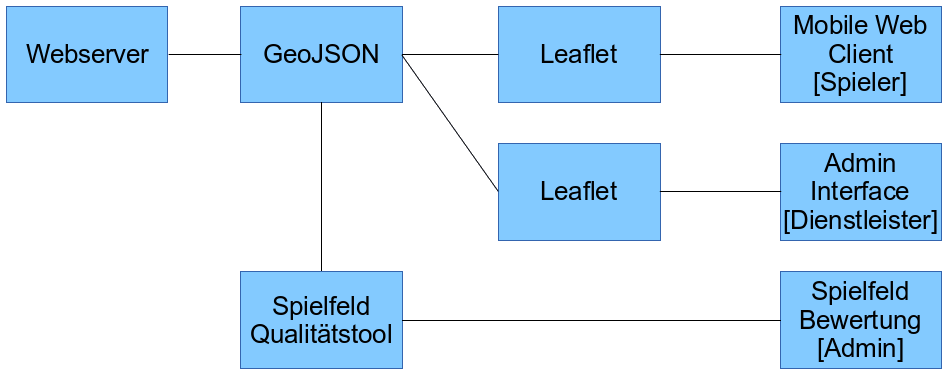
\includegraphics[width=140mm]{images/ch5_img04_interfaces.png}
\caption{Visualisierte Schnittstellen des Frameworks}
\label{img:ch5_img04_interfaces}
\end{center}
\end{figure}

Dadurch, dass das Framework die Daten von OSM/Overpass als JSON erhält und das Format bestens geeignet ist für den Austausch, da eine Vielzahl der aktuellen Frameworks und Tools dieses unterstützen ist die Wahl auf den Export der Spielelemente und Händlerdaten auf GeoJSON gefallen. Während das offene Format WKT für die reine Repräsentation von Geodaten dient \cite{Stolze.2003}, bietet das GeoJSON FOrmat zusätzlich die Möglichkeit entsprechende Properties an ein Geo Objekt zu speichern \cite{Butler.2008}. Über diese kann wiederum das Framework Informationen wie z.B. die codierte OSM ID und Informationen zum Spielelement übertragen.
\\\\
Generell werden die Informationen des Frameworks für drei verschiedene Module benötigt.
Zunächst einmal gibt es den Spielclient bzw. dessen Oberfläche. Dieser benötigt die Daten für das Staging des Spiels selbst.
Über die Spieloberfläche interagiert der Spieler mit dem Spiel. Er Sieht die aktuelle Karte, sowie die darauf platzierten Objekte. In diesem Fall sind dies die Spielelemente sowie die einzelnen Händler. Die Spielelemente selbst stellen im Beispielspiel die sogenannten Prestige Flaggen dar.
Ein weiteres Moduls stellt die Administartionsoberfläche dar. DIese dient dazu dem Spielleiter sowie dem jeweiligen Händler eine Konfiguration des Spiels vorzunehmen. Im Detail kann der Spielleiter die entsprechenden Spielitems definieren, neue Händler anlegen und diese auf der Karte positionieren. Der Händler kann seine Metadaten pflegen und entsprechende Items, welche er in seinem virtuellen Laden anbieten möchte selektieren und anbieten. Bei Fehlern oder Aktualisierungen kann der jeweilige Administrator (Spieleiter oder Händler) diese problemlos anpassen. Für die Positionierung der virtuellen Läden auf der Karte wird ebenfalls analog zum Spielfeld eine GeoJSON Schnittstelle zum Einsatz kommen.
Das letzte Modul stellt die Evaluierung der Spielfelder dar. Hier wird dem Spielleiter durch die Verwendung der gleichen Schnittstelle, wie für die Aufbereitung des Spielfeldes, die Möglichkeit geboten Daten in ein entsprechendes Evaluationstool mit entsprechendem Algorithmus  zu importieren. Dieses Tool wird entsprechend in Kapitel \ref{ch:CH6_qualtiy_of_gameboards} in vorgestellt. Über dieses wird das ideale Key-Value Paar für die OSM Tag Selektion der Daten evaluiert. Dies soll dem Spielleiter die Möglichkeit einer Objektiven Bewertung der Spielfelder ermöglichen.

\subsection*{Darstellung}

Da das Framework für ortsbezogene Spiele verwendet werden soll, ist es daher unerlässlich dem Spieler, sowie den Administratoren eine entsprechende Visualisierung zu bieten. Zunächst gibt es das Spielfeld. Das Spielfeld verwendet im Hintergrund Kartenmaterial von OSM, auf das die einzelnen Elemente platziert werden. Die Karte selbst wird initial auf die (GPS-)Korrdinaten der Spielerposition zentriert. Dadurch ist es dem Spieler möglich sich direkt von seiner Position aus zu Orientieren. Die auf der Karte eingezeichneten Eleemente wie Flaggen und Händler kann der Spieler somit problemlos identifizieren und zu Fuß aufsuchen. In Abbildung \ref{img:ch5_img05_dialog} ist ein Mockup der Kartenoberfläche zu sehen. Je nach Flaggestatus werden die Flaggen unterschiedlich farbig dargestellt. Das Ziel ist es Neutrale Flaggen grau, feindliche Rot und eigene grün darzustellen. Damit erhält der Spieler automatisch einen Überblick über die Situation und kann auch durch das Herauszoomen der Karte seine weiteren Spielzüge entsprechend planen.
Über die Elemente hinaus werden dem Spieler sein aktueller Punktestand. Dieser wird im Beispielspiel durch das einfache Addieren der Prestige der Flaggen die im Spielerbesitz sind berechnet. Des weiteren wird dem Spieler eine Auswahl für sein Inventar angezeigt werden. Über dieses kann er nicht nur sich alle Items in seinem Besitz anzeigen lassen, sondern auch diese verwenden und in einem späteren Ausbau des Frameworks Items mit anderen Spielern tauschen.
Sofern der Spieler mit einer Flagge interagiert, wird ihm die aktuelle Prestigezahl der Flagge angezeigt. Je nachdem ob ihm die Flagge bereits gehört oder diese einem fremden Spieler angehörig ist, kann der Spieler diese "angreifen". Durch den Angriff werden die Aktionspunkte des Spielers auf die Flagge transferiert. Ist die Flagge im Besitzt eines anderen Spielers so sieht der Spieler dies durch die aktuelle Farbgebung und kann durch den Einsatz seiner Aktionspunkte die Prestigezahl reduzieren, was direkt angezeigt wird. Für die Interaktion mit Händlern, steht dem Spieler ebenfalls ein Menü zur Verfügung, sobald er auf einen der Händler klickt. Danach öffnet sich ein Menü über das der Spieler eine Übersicht der verfügbarne Items sowie deren Spielpreise erhält. Sollte der Händler darüber hinaus Items wie in Kapitel \ref{ch4:s:choosen_solution} angedeutet mit Coupons arbeiten, so kann der Spieler diesen an gegebener Stelle eingeben.

\begin{figure}[H]
\begin{center}
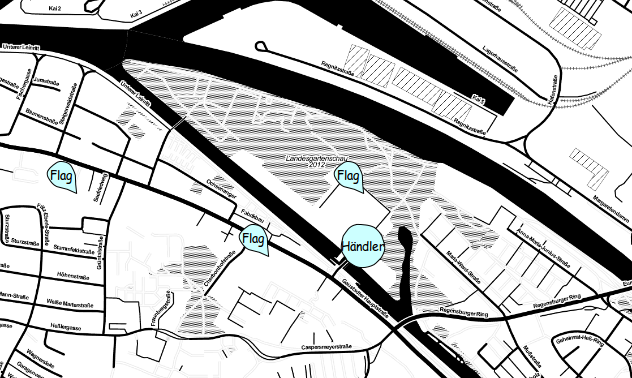
\includegraphics[width=140mm]{images/ch5_img05_dialog.png}
\caption{Spielfeld Mockup}
\label{img:ch5_img05_dialog}
\end{center}
\end{figure}

Der Administrationsbereich für den Spielleiter und den Händler arbeitet separat vom Spielfeld.
Je nachdem, ob Items oder Händler in das System gepflegt werden sollen, wird der Benutzer mit einer Liste präsentiert.
Im Fall der Items, erhält der Benutzer eine Übersicht über alle Items die dem Spiel zur Verfügung stehen. Hierbei handelt es sich allerdings nicht um Itemtypen sondern direkt um die instantiierten Items selbst. Die Idee dahinter ist es, dem Spiel die Möglichkeit zu bieten auch einzigartige Items zu enthalten und sicherzustellen, dass ein Item jeweils auch immer als solches im System behandelt wird. Über die Liste gibt es die Option die bestehenden Items zu modifizieren oder zu entfernen. Neue Items können übe reine Schaltfläche entsprechend angelegt werden. Dabei wird dem Benutzer eine entsprechende Oberfläche präsentiert und über Metadaten das Item genauer spezifiziert. Beispielsweise der Name, Itemtyp und der dafür  zu zahlende Preis.
\\\\
Möchte der Benutzer dahingegen Händler pflegen, so erhält er zunächst analog zu den Items eine Übersicht der einzelnen Händler.
Diese kann er analog zu den Items entsprechend modifizieren und löschen. Auch das Anlegen eines neuen Händlers ist analog zu den Items. Der Unterschied liegt jedoch drin, dass es sich bei den Händlern nicht um einfache Formularfelde rhandelt, sondern auch zusätzlich eine Georepräsentation stattfinden muss. D.h. es muss die Position des Händlers auf einer Karte erfolgen. Hierzu wird eine Art "Picker" verwendet. Auf einer OSM Karte soll der Benutzer die Position des Händlers definieren. Für eine Korrektur der Position reicht es aus, wenn der Benutzer einfach den Marker auf der Karte mit der Maus ergreift und per drag n drop auf seine neue Position bewegt.

%%\subsection*{Sonstige Funktionalitäten}


\subsection*{Technischer Entwurf}

Nachdem die Anforderungen beschrieben wurden, muss der Softwareteschnische Entwurf konkretisiert werden.
Um die Software entsprechend abzubilden zu können muss zunächst ein Modell entworfen werden, welche die Software abbildet. Die Prozesse des Frameworks wurden bereits in Abbildung \ref{img:ch5_img01_framework_progress} sowie \ref{img:ch5_img04_interfaces} visualisiert.

Zu Beginn einer Systementwicklung müssen die Usecases und die beteiligten Akteure identifiziert werden.
Hierfür wird zu Beginn überlegt, welche Personen Zugang zum System haben und welche Aufgaben diese am System erfüllen werden.
Dadurch wird sichergestellt, dass alle Aspekte behandelt werden, nicht nur die im initialen Lösungsansatz. Diese sind wichtig für den späteren Entwurf des Systems, sowie deren Umsetzung.
Die Usecases lassen sich als Diagramm wie in Abbildung \ref{img:ch5_img06_usecases} sichtbar definieren.



\begin{figure}[H]
\begin{center}
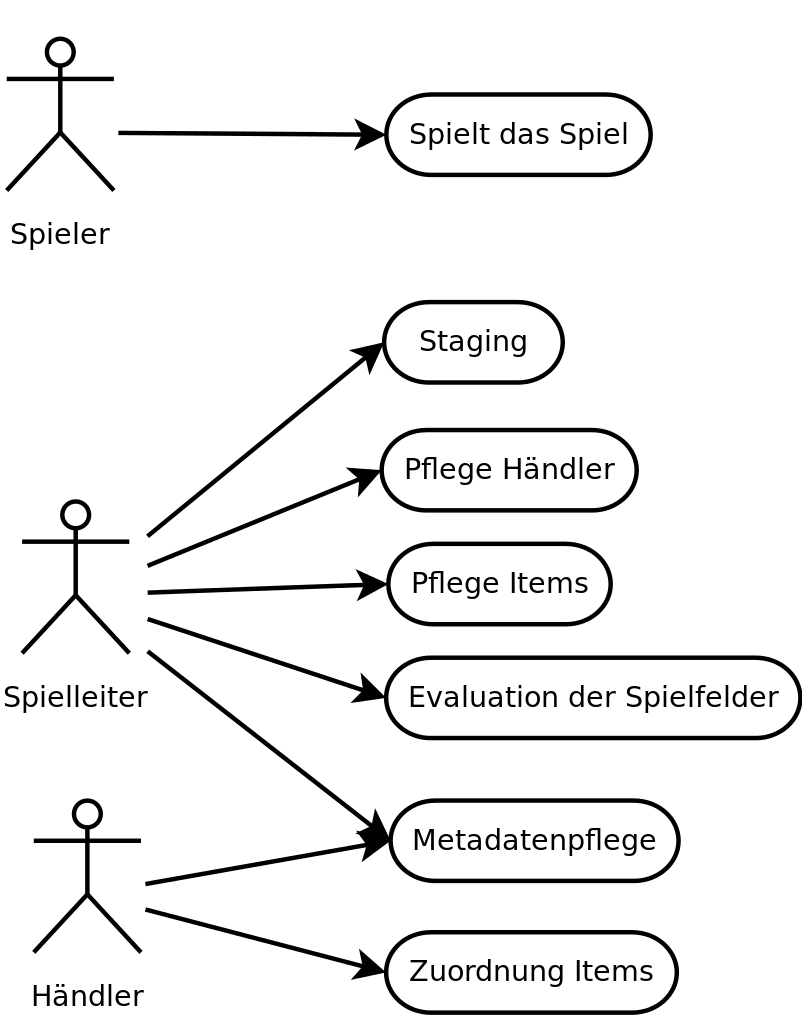
\includegraphics[width=100mm]{images/ch5_img06_usecases.png}
\caption{Usecase Diagramm}
\label{img:ch5_img06_usecases}
\end{center}
\end{figure}

Zunächst lässt sich feststellen, dass es drei Akteure gibt.
Diese decken sich soweit mit dem Lösungsansatz.
Der Spiele hat das Ziel das Spiel zu spielen. Der Spielleiter hingegen sieht es vor entsprechend das Staging des Spiels mit dem Framework zu bewerkstelligen.
Hier muss er die Händler als auch Items pflegen. Darüber hinaus teilt er sich mit dem Händler die Metadatenpflege, da je nach Situation der Spielleiter mehr oder weniger in die individuelle Pflege der Händlerdaten eingebunden ist. Der Händler möchte zusätzlich seine Items, die er vom Spielleiter zugewiesen bekommen hat entsprechend auf seine virtuellen Läden verteilen. In der Grundfunktion des Framesworks sind nur diese Benutzer vorgesehen. In einem Ausbau des Frameworks macht es Sinn explizite Nutzerrollen einzuführen um eine detailliertere Rechtezuweisung zu ermöglichen.
\\\\
Durch die Verwendung einer objektorientierten Programmiersprache ist es notwendig entsprechende Klassen zu definieren.
Diese dienen dazu, Objekte abzuleiten und die jeweiligen Methoden von diesen zu nutzen.
Es muss sichergestellt werden, dass die Beziehungen zwischen den Klassen modular sind, damit ein einfacher Zugriff und eine Austauschbarkeit gegeben ist.
Um ein Einblick in die Struktur des Frameworks zu erhalten wird in diesem Abschnitt kurz auf die wichtigsten Aspekte eingegangen.


\begin{figure}[H]
\begin{center}
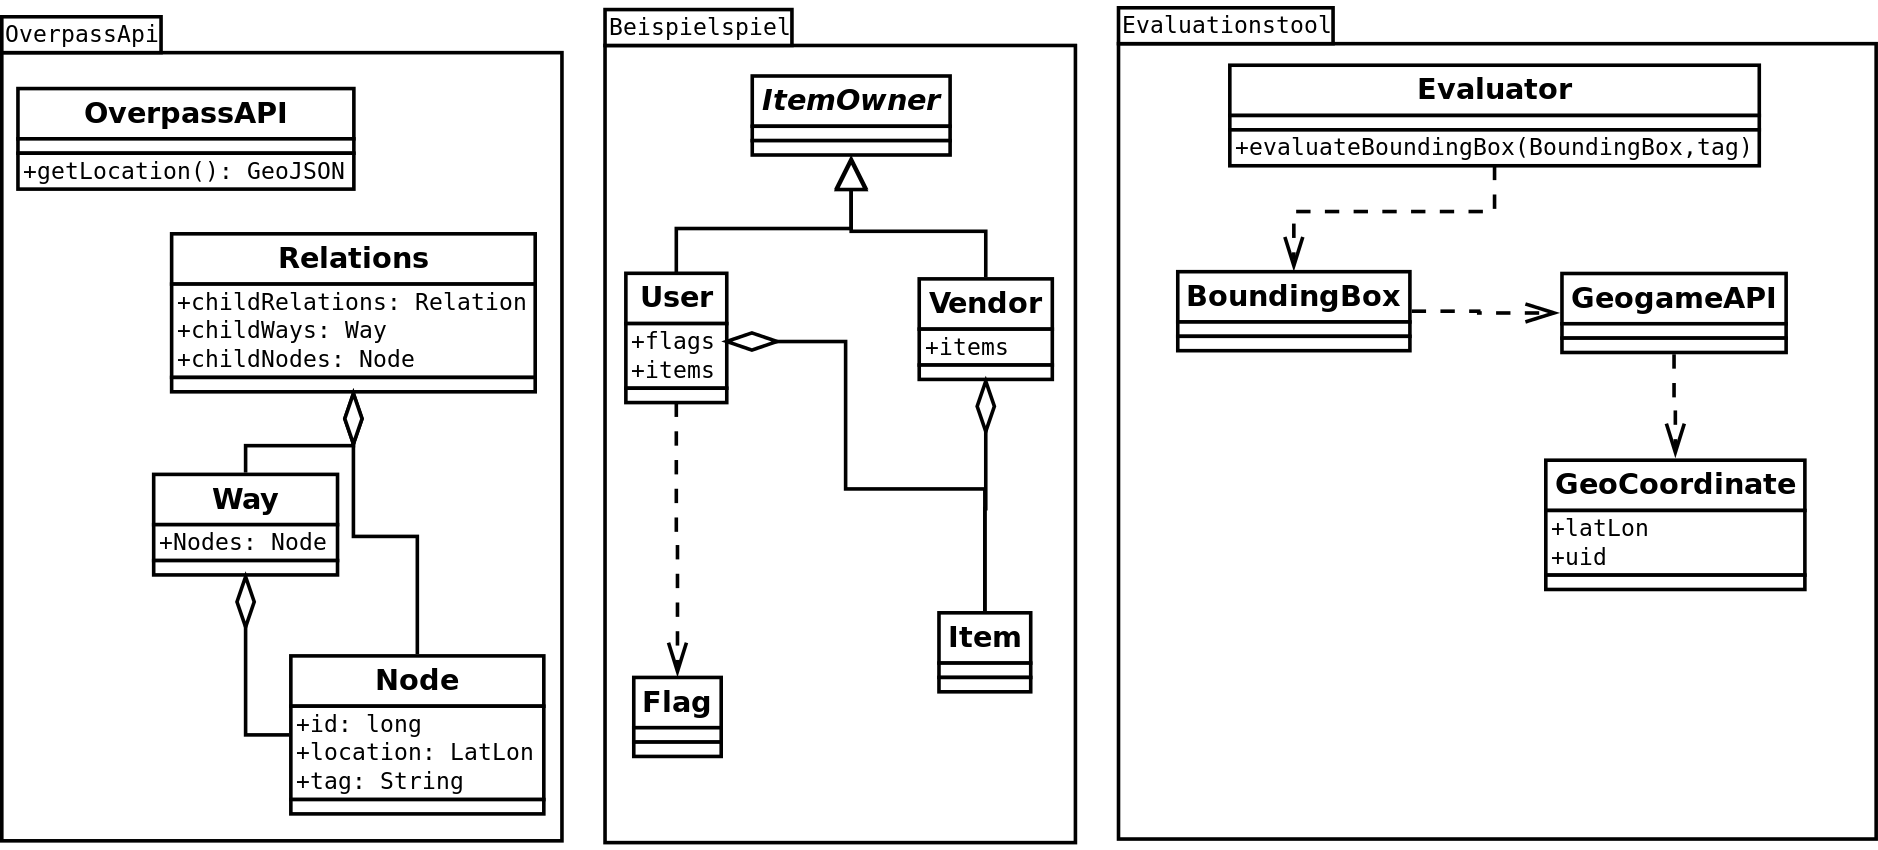
\includegraphics[width=150mm]{images/ch5_img07_classes.png}
\caption{Vereinfachtes Klassen Diagramm}
\label{img:ch5_img07_classes}
\end{center}
\end{figure}

In Abbildung \ref{img:ch5_img07_classes} ist ein vereinfachtes Klassendiagramm des Frameworks zu sehen. Das Framework als solches besteht aus drei Modulen. Zunächst gibt es den Bereich \textit{OverpassApi}. Hierbei handelt es sich nicht um die OverpassApi selbst, da Overpass selbst nur eine Webschnittstelle ist, sondern um die Implementierung einer entsprechenden Schnittstelle im Framework selbst, welches das Ergebnis der OverpassApi im Web transferiert auf die einzelnen Elemente Relations, Ways und Nodes. Diese werden wiederum durch den bereits beschriebenen Ansatz entsprechend transformiert in dem eine umcodierung in virtuelle Nodes erfolgt. Im gleichen Zug wird überprüft, ob es persistierte Daten für die virtuellen Nodes in der lokalen Datenbank gibt. Ist dem der Fall, so werden die virtuellen Nodes um die entsprechenden Properties ergänzt und anschließend als JSON bzw. GeoJSON gerendert.
Im Anschluss werden diese über die Webschnittstelle des eigenen Frameworks ausgegeben.
Für die Händler gibt es eine separate Schnittstelle im Framework, welche analog zur Overpass Implementierung fungiert, aber hierbei nicht die Daten von extern (OSM/Overpass) bezieht, sondern direkt in der fertigen Form aus der lokalen Datenbank auslesen kann. Hierbei ist zudem auch keine entsprechende Transformation notwendig, sondern diese liegen bereits als fertige Nodes vor. Dies ist möglich, da jeder Händler nur als einziger Punkt im Spiel repräsentiert wird.
\\\\
Das nächste Modul ist das \textit{Beispielspiel}. Das Beispielspiel selbst wurde einfach gehalten, da es zum einen als Proof of Conecept des Frameworks dienen soll, zum anderen der Fokus auf die Verteilung der Spielelemente auf dem Spielbrett untersucht werden soll.
Generell gibt es 4 Objekte. \textit{Spieler}, \textit{Händler}, \textit{Flaggen} und \textit{Items}.
Spieler und Händler stehen in einer polymorphen Verbindung zu Item. Ausgelöst, leiten beide Klassen von einer abstrakten Klasse \textit{ItemOwner} ab, welche entsprechende Methoden vorhält die für die Interaktion als ItemOwner essentiell sind. Beispielsweise der Verkauf oder die Benutzung eines Items. Ein Item kann nur einem Spieler oder einem Händler angehören, niemals aber beiden gleichzeitig. Des weiteren gibt es auch die Möglichkeit, dass ein Item ohne ItemOwner existiert. Ein Beispiel könnte es sein, dass der Spielleiter für ein Event bestimmte Items auf der Karte ablegt oder lokale zwei Spieler Items manuell tauschen möchten.
\\\\
Das letzte Modul stellt das sogenannte \textit{Evalutationstool} dar.
Mit diesem sollen die erzeugten Spielfelder analysiert und bewertet werden. Eine genauere Erläuterung ist in Kapitel \ref{ch:CH6_qualtiy_of_gameboards} zu finden.
Das Evaluationstool gereift zunächst auf die GeoJSON Schnittstelle des Frameworks zu. Dieses liefert bei entsprechender Abfrage mittels Bounding Box und entsprechendem OSM Tags die Spielelemente zurück. Die Boundingbox wird auf Basis einer initialen Koordinate berechnet. Somit kann der Spielleiter einfach zwei Koordinaten definieren zu denen er gerne eine entsprechende Auswertung interessanter Tags erhalten möchte. Das Evaluationstool startet im Anschluss den Vorgang und wandelt die Spielelemente in vereinfachte Objekte mit ID und Geo-Kooridnaten um. Diese wiederum werden der jeweiligen Evaluationsmethode als Liste übergeben und deren Rückgabewert beschreibt die Kombination aus Boundingbox und OSM Tag.

\subsubsection*{Datenbank}

Aufgrund der vorherigen Analysen wird normalerweise ein Enitity Relationship Model (ERM) erstellt. Allerdings soll der Einsatz eines Webframeworks erfolgen welches ein mindestens ein Objektrelationales Mapping unterstützt und somit die Manuelle Erstellung der Datenbankstruktur nicht mehr vorgesehen ist. Dies wird unter der Annahme gemacht, dass das Framework später im Produktiv Betrieb für die Datenspeicherung optional auf eine NoSQL Lösung umgestellt werden kann. Diese bieten eine bessere Performance bei einfachen Abfragen.
Dies geschieht auch vor dem Hintergrund den in der Literatur häufig kritisierten Mismatch zwischen Objektorientierter Programmierung und der Verwendung von Relationalen Datenbanken um Objekte welche von Klassen abgeleitet wurden zu speichern \cite{Cattell.1991}.

Die geringe Verbreitung der objektorientierten Datenbanken liegt darin, dass nicht
versucht wurde die bestehenden Datenbanken zu ersetzten. Viel mehr sind die bereits existierenden Datenbanken in Unternehmen nicht in neue objektorientierte Datenbanken transferiert worden. Der Grund hierfür liegt in den historisch gewachsenen Applikationen und Datenbanken, dessen Umstellung einen sehr hohen Aufwand und Kosten darstellen würde \cite{Burleson.1994}.

Ein weiter Aspekt ist die Tatsache, dass die objektorientierten Datenbanken nicht in jedem Aspekt
besser sind als relationale Datenbanken. Es gibt Situationen in denen haben Objektorientierte
Datenbank Management Systeme klare Vorteile gegenüber den relationalen Datenbanken besitzen.
Die Objektorientierten Datenbanken spielen Ihre Vorteile speziell bei der Abbildung
von Beziehungen von Objekten untereinander aus. Nicht nur bei Vererbungen sondern auch wenn
die Objekte diverse Methoden besitzen. Bei einer Sequentiellen Abfrage mehrerer Datensätze sind
jedoch die relationalen im Vorteil \cite{Van.2006}. Hier ist es notwendig den Zweck der zu speichernden Daten bzw. deren Verwendung zu untersuchen. Je nachdem kann der Einsatz von objektorientierten Datenbanken oder relationalen Datenbanken Sinn machen.

Vergleicht man die Verbreitung von objektorientierten Datenbanken in gewissen Einsatzgebieten, so lässt sich feststellen, dass diese trotz der in Summe geringen Verbreitung ein berechtigtes Dasein haben. Speziell in Geoinformationssystemen spielen objektorientierte Datenbank Management Systeme ein wichtige Rolle,\cite{Brinkhoff.2005} da Sie deutlich einfacher ermöglichen komplexe Verbindungen zwischen den unterschiedlichen Objekten herzustellen und eine Veränderung dieser Beziehungen in einem Bruchteil der Zeit ermöglichen, welcher eine relationale Datenbank dafür aufwenden müsste. Die umfangreiche Literatur zum Thema Geoinformationsysteme gibt einen Ausblick für Möglichkeiten sich durch die Nutzung dieser ergeben können.

\subsection*{Weitere Aspekte}

Ein weiterer Aspekt stellt die Optimierung der Anfragen an die Overpass Api Schnittstelle des Frameworks seitens des Spielfeldes dar. In der Grundvariante des Frameworks, stellt das Spielfeld jeweils eine Anfrage als Bounding Box an die Schnittstelle um die aktuellen Spielelemente für den aktuellen Kartenausschnitt zu erhalten.

%% performance messungen?

\section{Bewertung der Technologien und Werkzeuge}

-Webframework
-Kartendarstellung
-Schnittstellen

\section{Implementierung des Geogameframeworks}



\subsubsection*{Probleme}